\documentclass[12pt,a4paper]{amsart}

\usepackage[slovene]{babel}
\usepackage[T1]{fontenc}
\usepackage[utf8]{inputenc}
\usepackage{amsmath,amssymb,amsfonts}
\usepackage{url}
\usepackage{graphicx}
\usepackage{subcaption}
\usepackage{float}
\usepackage[dvipsnames,usenames]{color}
\usepackage{hyperref}
\hypersetup{
     colorlinks   = true,
     citecolor    = gray
}

\graphicspath{ {./slike/} } % Watch out
\textwidth 15cm
\textheight 24cm
\oddsidemargin.5cm
\evensidemargin.5cm
\topmargin-5mm
\addtolength{\footskip}{10pt}
\pagestyle{plain}
\overfullrule=15pt % oznaci predlogo vrstico

% ukazi za matematicna okolja
\theoremstyle{definition} % tekst napisan pokoncno
\newtheorem{definicija}{Definicija}[section]
\newtheorem{primer}[definicija]{Primer}
\newtheorem{opomba}[definicija]{Opomba}

\renewcommand\endprimer{\hfill$\diamondsuit$}


\theoremstyle{plain} % tekst napisan posevno
\newtheorem{lema}[definicija]{Lema}
\newtheorem{izrek}[definicija]{Izrek}
\newtheorem{trditev}[definicija]{Trditev}
\newtheorem{posledica}[definicija]{Posledica}

% za stevilske mnozice uporabi naslednje simbole
\newcommand{\R}{\mathbb R}
\newcommand{\N}{\mathbb N}
\newcommand{\Z}{\mathbb Z}
\newcommand{\C}{\mathbb C}
\newcommand{\Q}{\mathbb Q}

% ukaz za slovarsko geslo
\newlength{\odstavek}
\setlength{\odstavek}{\parindent}
\newcommand{\geslo}[2]{\noindent\textbf{#1}\hspace*{3mm}\hangindent=\parindent\hangafter=1 #2}

% ' Tu se zacne '
\newcommand{\program}{Finančna matematika} % ime studijskega programa: Matematika/Finan"cna matematika
\newcommand{\imeavtorja}{Urh Peček, Jan Škoberne} % ime avtorja
\newcommand{\imementorja}{prof. dr. Riste Škrekovski , asist. dr. Janoš Vidali} % akademski naziv in ime mentorja
\newcommand{\naslovdela}{Traveling salesman problem} % Naslov dela
\newcommand{\letnica}{2019} %letnica 


\begin{document}

\thispagestyle{empty}
\noindent{\large
UNIVERZA V LJUBLJANI\\[1mm]
FAKULTETA ZA MATEMATIKO IN FIZIKO\\[5mm]
\program\ -- 1.~stopnja}
\vfill

\begin{center}{\large
Avtorja: \imeavtorja\\[2mm]
{\bf \naslovdela}\\[10mm] 
Mentorja: \imementorja\\[2mm]

Projekt pri predmetu Operacijske raziskave\\[1cm]}

\end{center}
\vfill

\noindent{\large
Ljubljana, \letnica}
\pagebreak

\thispagestyle{empty}
\hypersetup{linkcolor = black}
\tableofcontents
\pagebreak

\section{Navodilo}
\bigskip
We would like to deal with metric version of Traveling Salesmen Problem. First, implement the an algorithm to solve the minimum weighted spanning tree problem, and afterwards, implement Double-Tree Algorithm and Christofides’ Algorithm for metric TSP using the previous algorithm. Then compare both algorithms for various instances of TSP. As test data, use both Euclidean and non-Euclidean instances. 
\bigskip

\centerline{\large Navodilo v slovenščini:} 
\bigskip
Želeli bi se ukvarjati z metrično različico problema potujočega trgovca.
Najprej izvedite algoritem za reševanje problema za drevo z minimalno težo, nato pa izvedite algoritem z dvojnim drevesom in Christofidesov algoritem za metrični TSP z uporabo prejšnjega algoritma. Nato primerjajte oba algoritma za različne primere TSP. Kot preskusne podatke uporabite evklidske in neevklidske primerke.

\newpage
\section{Predstavitev problema} 

Najina naloga je bila obravnava problema \textbf{potujočega trgovca} v metrični različici.
\newline
Pri problemu potujočega trgovca se vprašamo, katera je glede na seznam mest in danih razdalj med mesti, najkrajša pot, ki obšče vsa mesta in se vrne v prvotno. 
To je NP-težek problem, torej problem pri katerem lahko učinkovito preverimo, ali je rešitev pravilna, vendar za reševanje ne poznamo učinkovitih algoritmov in ne verjamemo da obstajajo. \\
Na splošno velja, da ima vsak utežen usmerjen graf (ne nujno povezan) gozd z minimalno težo, kar je združitev dreves z minimalno težo za njegove povezane sestavne dele.
\\
\newline
Algoritem za \textbf{reševanje problema za drevo z minimalno težo} nam vrne točno vrednost najkrajše poti potujočega trgovca  v danem grafu, vendar je običajno ta algoritem časovno prezahteven, zato njegovo vrednost aproksimiramo. 
V našem primeru smo za aproksimacijo izbrali \textbf{Double tree algoritem}t in\textbf{Christofidiesov algoritem}.
Primerjala sva njuno časovno zahtevnost ter napako pri iskanju najkrajše poti.
\bigskip

\newpage
\section{Pristop h reševanju problema}

Naloge sva se seveda lotila reševati grafično. Kot programski jezik sva uporabljala Sage na platformi Cocalc. \newline 
Posamezna mesta sva predstavila z vozlišči grafa, razdalje med mesti pa z uteženimi povezavami med vozlišči.  Gre za težavo z minimizacijo, ki se začne in konča v določeni točki, potem ko smo vmes obiskali vsa druga vozlišča grafa natančno enkrat.
Iskala sva torej najkrajši Hamiltonov cikel v danem grafu.
\hfil\\\

Kot prvo sva sestavila algoritem za reševanje problema za drevo z minimalno težo. \textbf{Drevo z minimalno težo je} podmnožica povezav povezanega, obteženega (uteži na povezavah) grafa, ki povezuje vsa vozlišča, je brez ciklov in ima najmanjšo skupno težo povezav.
Ta algoritem nam da točno rešitev problema za določen graf. Nato sva napisala še Double tree algoritem in Christofidiesov algoritem.
\\
Na začetku sva vse tri algoritme napisala posebej, kasneje pa jih spremenila v en sam algoritem znotraj funkcije s pomočjo katere sva izvajala teste.
Za rezultate algoritmov sva ustvarila še posebno funkcijo, ki nama je omogočala preprost zapis podatkov v csv datoteko in kasneje v Excel, kjer sva kasneje tudi ustvarila grafe za boljšo predstavo rezultatov.

\newpage
\section {Predstavitev algoritmov} 

Natančno predstavitev algoritmov si lahko ogledamo prek kode, ki je dodana na Githubu. \\
Za \textbf{merjenje časovne zahtevnosti} algoritmov sva uporabljala funkcijo $time.time()$\\
Čas, ki ga algoritem porabi za izračun sva izmerila kot časovno razliko med začetkom in zaključkom izvajanja algoritma.
\bigskip

Pri vseh treh algoritmih najprej ustvarimo graf. Vso testiranje izvedemo pri različnih vrstah teh grafov, na katerih temelji tudi celotna funkcija, ki jo poženemo kot test. 
Določimo lahko dimenzijo grafa, interval s katerega jemljemo točke in število točk, torej vozlišč v grafu.
\bigskip


\subsection{Algoritem za iskanje drevesa z minimalno težo} \hfill\\

V grafu z n vozlišči ima vsako drevo n-1 povezav.
V danem grafu je lahko več dreves z minimalno težo zlasti, zlasti so teže vseh povezav grafa enake, posledično je vsako drevo v grafu minimalno.
Skoraj gotovo v nobenem testu nismo dobili grafa, kjer bi imele vse povezave enake teže, skoraj gotovo ni niti dveh takih povezav, saj smo težo povezave dobili z razdaljo med točkama v prostoru, ki je bila določena naključno z realnega intervala, ki smo ga določili v glavni funkciji.
\newline
Če so vse uteži pozitivne, kar v našem primeru so, potem je drevo z minimalno težo  v resnici podgraf z minimalnimo težo, ki povezuje vse točke, saj morajo podgrafi, ki vsebujejo cikle, nujno imeti večjo težo.
\hfill\\\

V najinem primeru sva za izračun najkrajše poti v naključno ustvarjenem grafu uporabila v Sage-u že ugrajeno funkcijo $Travelling\_salesman\_problem()$.
Ta nam je vrnila graf z minimalno težo, v katerem smo za izračun točne vrednosti najkrajše poti v danem grafu zgolj še sešteli uteži na povezavah.
Kot rečeno nam ta algoritem vrne točno vrednost najkrajše poti v danem grafu in je časovno najbolj zahteven.
Kot osnovno za ostala dva algoritma sva uporabljala zgornjega in glede na njegov rezultat ugotavljala njuno natančnost.
\\hfil\\\

\textbf{Algoritem dvojnega drevesa in Christofidiesov algoritem} oba temeljita na Eulerjevi poti iz katere postopoma odstranjujemo vozlišča.
Razlikujeta se, glede na to kako je utežena Eulerjeva pot ustvarjena. Double tree algoritem podvoji vsako povezavo v drevesu z minimalno težo, kjer pa Christofidiesov algoritem drevesu z minimalno težo doda vozlišča s sodo stopnjo.

\subsection{Double tree algoritem} \hfill\\\

Double tree algoritem je torej eden od algoritmov, ki vrne približek točne vrednosti dolžine najkrajše poti, ki obišče vsa vozlišča grafa natanko enkrat.
Double tree algoritem zagotavlja, da bodo njegove rešitve znotraj faktorja 2 optimalne dolžine rešitve\\
Vemo, da ima graf Eulerjev sprehod, če je vsako vozlišče sode stopnje. Zato je za rešitev TSP dovolj, da najdemo najcenejši podgraf v katerem je vsako vozlišče sode stopnje.
V Double tree algoritmu to storimo s podvojitvijo vsake povezave v drevesu z minimalno težo.
\hfil\\\

\textbf{Double tree algoritem}: 
\begin{description}
 \item[Vhod] Utežen graf $(K_n,c)$ na katerem iščemo najkrajšo pot.
 \item[Izhod] Hamiltonov cikel $H$ in najkrajša pot.
 \item[Algoritem]
\end{description}
\begin{itemize}
\item Pošči drevo z minimalno težko $T$ v grafu $K_n$;
\item Podvoji vse povezave v drevesu $T$ in poišči Eulerjev sprehod $L$;
\item Pretvori Eulerjev sprehod $L$ v Hamiltonov cikel $H$ v prvotnem grafu $K_n$;
\end{itemize}
\hfil
\begin{itemize}
\item[Opomba:] Eulerjev sprehod je sprehod, ki obišče vsako vozlišče grafa natanko enkrat.
\end{itemize}

\subsection{Christofidiesov algoritem} \hfill\\\

Drug način s katerim iščemo najkrajšo trgovčevo pot v danem grafu je torej Christofidiesov algoritem.
Gre za algoritem približevanja, ki zagotavlja, da bodo njegove rešitve znotraj faktorja 3/2 optimalne dolžine rešitve in je poimenovan po Nicosu Christofidesu, ki ga je objavil leta 1976.
Od leta 2019 je to najboljše približevalno razmerje, ki je bilo dokazano za problem potujočega prodajalca na splošnih metričnih prostorih, čeprav so za nekatere posebne primere boljši drugi približki. \\

\textbf{Christofidiesov algoritem:}
\begin{description}
 \item[Vhod] Utežen graf $(K_n,c)$ na katerem iščemo najkrajšo pot.
 \item[Izhod] Hamiltonov cikel $H$ in najkrajša pot.
\end{description}
\begin{itemize}
\item Pošči drevo z minimalno težko $T$ v grafu $K_n$;
\item Naj bo $W$ množica vozlišč z sodo stopnjo v drevesu $T$;
\item Poišči minimalno ujemanje vozlišč $M$ v $W$, v grafu $K_N$;
\item Združi povezave v $M$ in $T$ , tako da tvorijo povezan multigraf $V$, v katerem poišči Eulerjev sprehod $L$;
\item Pretvori Eulerjev sprehod $L$ v Hamiltonov cikel $H$ v prvotnem grafu $K_n$;
\end{itemize}

\newpage
\section{Ugotovitve} \hfill\\\

Spodaj sledi kratka predstavitev dobljenih rezultatov, več grafov in ugotovitev pa je v posebni mapi, ki je priložena na Github repozitoriju.
\\
\begin{figure}[h!]
  \centering
    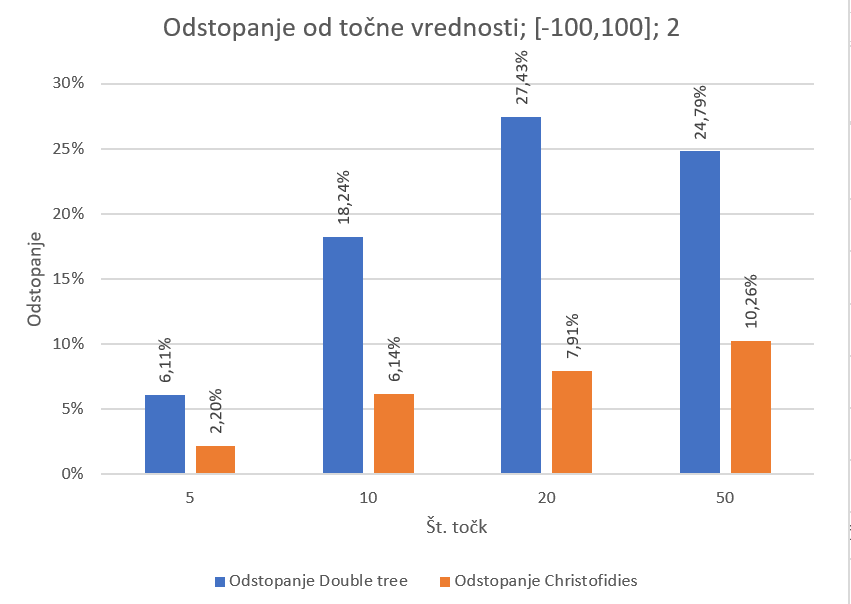
\includegraphics[width=\linewidth]{OdstopanjeOverall.PNG}
    \caption{Povprečno odstopanje od točne vrednosti pri različnem številu točk z intervala [-100,100] in grafa v 2. dimenziji.}
\end{figure}

Kot zanimivost lahko opazimo, da pri algortimu Double tree pride do največjega odstopanja pri 20 točkah, kar je v nasprotju z našimi pričakovanji.
Število ponovitev je bilo precejšnje zato dvomiva, da je to naključje.
Sicer pa lahko potrdimo zgoraj povedano, da je Christofidiesov algoritem precej bolj natančen kot algoritem Double tree.
Morda je zanimivo tudi, da je pri 5., 10. in 20. točkah napaka double tree algoritma približno 3-krat večja od napake Christofidiesovega algoritma, medtem, ko se pri 50. točkah ta razlika nekoliko zmanjša.

\newpage

\begin{figure}[h!]
  \centering
    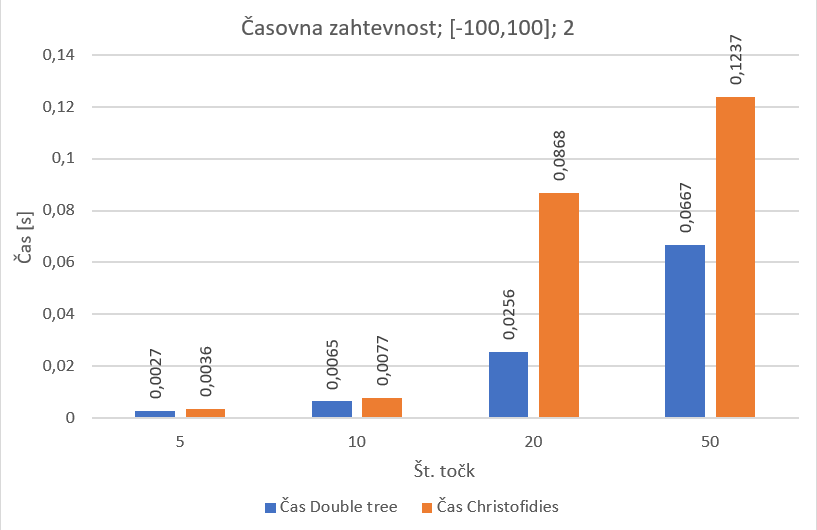
\includegraphics[width=\linewidth]{CasOverall.PNG}
    \caption{Povprečno trajanje izvedbe algoritma z različno število točkami z intervala [-100,100] in grafa v 2. dimenziji.}
\end{figure}

Opazimo, da je časovna zahtevnost Christofidiesovega algortima večja kot pri algoritmu Double tree. Torej ravno obratno kot pri odstopanju od točne vrednosti.
Pride tudi do znatnega povečanja trajanja pri skoku iz 10 na 20 točk, pri čemer je pri skoku z 20 na 50 točk razlika v trajanju izvedbe algoritma precej manjša, predvsem je to opazno pri Christofidiesovem algoritmu. 
\hfill\\\

Zaključimo lahko, da je Christofidieosv algoritem veliko bolj natančen kot algoritem double tree, vendar pa porabi precej več časa, zato se moramo pred uporabo odoločiti kaj nam je pomembneje, večja natančnost ali skrajšan čas izvedbe.


\end{document}





















